\documentclass[t,14pt]{beamer}
\usepackage{ep-dark}   % JHU/WSE style for use on Lightboard
\usepackage{graphicx}  % for inclusion of graphics
\usepackage{amsmath}   % good for additional math
\usepackage{amsthm}    % theorems, definitions, etc

% Keep diagrams in a directory named "figures"
% (Not used in this simple example.)

% \graphicspath{{./figures/}}  

\begin{document}


% These commands create the first slide
% \coursename specifies the name of the course. No need to include the
% course number especially since they change from time to time
%
% \modulename is the name of this particular lesson

\coursename{Introduction to Beamer for the Lightboard}
\modulename{Beamer Basics}
\titleframe


\begin{frame}
  \frametitle{Beamer}
  \large 

  We use \alert{Beamer} instead of PowerPoint to create presentations
  to be projected on a screen. Since it is based on \LaTeX, it is
  excellent for presentations with mathematical formulas.

  Indeed, we assume the user is already familiar with \LaTeX.
\end{frame}

\begin{frame}
  \large

  This slide deck uses the \texttt{ep-dark} style which provides a
  particularly simple, clean design featuring white text on a black
  backgound. This is ideal for use on the Lightboard.

  Keep it clean! Don't put too many words on a slide.
\end{frame}


\begin{frame}
  \frametitle{Blocks}
  \large
  \begin{block}{This is a block}
    A \alert{block} structure is useful for highlighting particular
    information.
  \end{block}

  \begin{definition}
    The \alert{definition} environment is a type of block used for
    definitions. Highlight the word you are defining.
  \end{definition}
\end{frame}

\begin{frame}
  \frametitle{Itemized lists}
  \large
  \begin{itemize}
  \item<+-> Itemized lists are useful for sequential points.
  \item<+-> In this example, each item appears on subsequent slides.
  \item<+-> Items are added one by one until done. 
  \end{itemize}
\end{frame}

\begin{frame}
  \frametitle{Pauses}
  \Large The \alert{pause} command 
  \pause 
  is a mechanism for building up a slide in pieces.
\end{frame}


\begin{frame}
  \frametitle{Only}
  \large  

  The \alert{only} command provides more fine control in revealing
  material on a slide.

  \only<2>{
    This sentence will only appear after the first the first one.
  }

  \only<3->{
    The second sentence was only on the $2^{\text{nd}}$ slide; this
    sentence will be on slides 3 and all subsequent slides.
  }

  \only<4>{
    Finally, this sentence appears.
  }

\end{frame}

\begin{frame}
  \frametitle{Mathematics}
  \large
  Because Beamer is built in \LaTeX\ it does mathematics beautifully
  either inside a sentence, $\sqrt2 + \cos\theta$, or in display mode:
  \[
  x = \frac{-b \pm \sqrt{b^2-4ac}}{2a} .
  \]

  Do it right! Notice this difference between $cos\theta$ [wrong!] and
  $\cos\theta$ [yes!]. 
\end{frame}

\begin{frame}
  \frametitle{Aligned equations}
  \large The \alert{aligned} environment (in math mode) works well
  with Beamer and pauses:
  \[
  \begin{aligned}
    |z| &= \sqrt{z \cdot \overline{z}} \\[12pt]
    \pause
    \therefore |a+bi| &= \sqrt{(a+bi)(a-bi)} \\ \pause
    &= \sqrt{a^2 +abi -abi - b^2i^2} \\ \pause
    &= \sqrt{a^2 + b^2}
  \end{aligned}
  \]
\end{frame}

\begin{frame}
  \frametitle{Figures}
  \large 
  The \alert{graphicx} package provides the \alert{includegraphics}
  command. Prepare graphics with a drawing program using light colored
  lines and shapes on a black or transparent background. Save in a
  standard graphics format.
  \begin{center}
    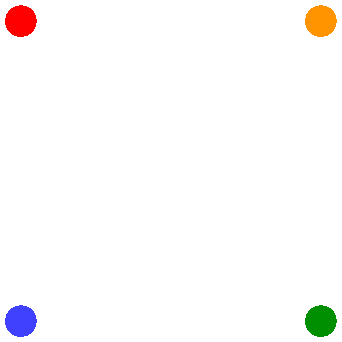
\includegraphics[scale=0.5]{figure}
  \end{center}
\end{frame}

\begin{frame}
  \frametitle{Math extras}
  \large
  Use the \alert{amsmath} and \alert{amsthm} packages for additional
  math functionality.

  \begin{theorem}[Binomial]
    Let $n$ be a nonnegative integer. Then
    \[
    (x+y)^n = \sum_{k=0}^n \binom{n}{k} x^k y^{n-k}. \qed
    \]
  \end{theorem}
\end{frame}


\end{document}
